\documentclass[
  man,
  floatsintext,
  longtable,
  nolmodern,
  notxfonts,
  notimes,
  colorlinks=true,linkcolor=blue,citecolor=blue,urlcolor=blue]{apa7}

\usepackage{amsmath}
\usepackage{amssymb}



\usepackage[bidi=default]{babel}
\babelprovide[main,import]{english}


% get rid of language-specific shorthands (see #6817):
\let\LanguageShortHands\languageshorthands
\def\languageshorthands#1{}

\RequirePackage{longtable}
\RequirePackage{threeparttablex}

\makeatletter
\renewcommand{\paragraph}{\@startsection{paragraph}{4}{\parindent}%
	{0\baselineskip \@plus 0.2ex \@minus 0.2ex}%
	{-.5em}%
	{\normalfont\normalsize\bfseries\typesectitle}}

\renewcommand{\subparagraph}[1]{\@startsection{subparagraph}{5}{0.5em}%
	{0\baselineskip \@plus 0.2ex \@minus 0.2ex}%
	{-\z@\relax}%
	{\normalfont\normalsize\bfseries\itshape\hspace{\parindent}{#1}\textit{\addperi}}{\relax}}
\makeatother




\usepackage{longtable, booktabs, multirow, multicol, colortbl, hhline, caption, array, float, xpatch}
\setcounter{topnumber}{2}
\setcounter{bottomnumber}{2}
\setcounter{totalnumber}{4}
\renewcommand{\topfraction}{0.85}
\renewcommand{\bottomfraction}{0.85}
\renewcommand{\textfraction}{0.15}
\renewcommand{\floatpagefraction}{0.7}

\usepackage{tcolorbox}
\tcbuselibrary{listings,theorems, breakable, skins}
\usepackage{fontawesome5}

\definecolor{quarto-callout-color}{HTML}{909090}
\definecolor{quarto-callout-note-color}{HTML}{0758E5}
\definecolor{quarto-callout-important-color}{HTML}{CC1914}
\definecolor{quarto-callout-warning-color}{HTML}{EB9113}
\definecolor{quarto-callout-tip-color}{HTML}{00A047}
\definecolor{quarto-callout-caution-color}{HTML}{FC5300}
\definecolor{quarto-callout-color-frame}{HTML}{ACACAC}
\definecolor{quarto-callout-note-color-frame}{HTML}{4582EC}
\definecolor{quarto-callout-important-color-frame}{HTML}{D9534F}
\definecolor{quarto-callout-warning-color-frame}{HTML}{F0AD4E}
\definecolor{quarto-callout-tip-color-frame}{HTML}{02B875}
\definecolor{quarto-callout-caution-color-frame}{HTML}{FD7E14}

%\newlength\Oldarrayrulewidth
%\newlength\Oldtabcolsep


\usepackage{hyperref}




\providecommand{\tightlist}{%
  \setlength{\itemsep}{0pt}\setlength{\parskip}{0pt}}
\usepackage{longtable,booktabs,array}
\usepackage{calc} % for calculating minipage widths
% Correct order of tables after \paragraph or \subparagraph
\usepackage{etoolbox}
\makeatletter
\patchcmd\longtable{\par}{\if@noskipsec\mbox{}\fi\par}{}{}
\makeatother
% Allow footnotes in longtable head/foot
\IfFileExists{footnotehyper.sty}{\usepackage{footnotehyper}}{\usepackage{footnote}}
\makesavenoteenv{longtable}

\usepackage{graphicx}
\makeatletter
\newsavebox\pandoc@box
\newcommand*\pandocbounded[1]{% scales image to fit in text height/width
  \sbox\pandoc@box{#1}%
  \Gscale@div\@tempa{\textheight}{\dimexpr\ht\pandoc@box+\dp\pandoc@box\relax}%
  \Gscale@div\@tempb{\linewidth}{\wd\pandoc@box}%
  \ifdim\@tempb\p@<\@tempa\p@\let\@tempa\@tempb\fi% select the smaller of both
  \ifdim\@tempa\p@<\p@\scalebox{\@tempa}{\usebox\pandoc@box}%
  \else\usebox{\pandoc@box}%
  \fi%
}
% Set default figure placement to htbp
\def\fps@figure{htbp}
\makeatother


% definitions for citeproc citations
\NewDocumentCommand\citeproctext{}{}
\NewDocumentCommand\citeproc{mm}{%
  \begingroup\def\citeproctext{#2}\cite{#1}\endgroup}
\makeatletter
 % allow citations to break across lines
 \let\@cite@ofmt\@firstofone
 % avoid brackets around text for \cite:
 \def\@biblabel#1{}
 \def\@cite#1#2{{#1\if@tempswa , #2\fi}}
\makeatother
\newlength{\cslhangindent}
\setlength{\cslhangindent}{1.5em}
\newlength{\csllabelwidth}
\setlength{\csllabelwidth}{3em}
\newenvironment{CSLReferences}[2] % #1 hanging-indent, #2 entry-spacing
 {\begin{list}{}{%
  \setlength{\itemindent}{0pt}
  \setlength{\leftmargin}{0pt}
  \setlength{\parsep}{0pt}
  % turn on hanging indent if param 1 is 1
  \ifodd #1
   \setlength{\leftmargin}{\cslhangindent}
   \setlength{\itemindent}{-1\cslhangindent}
  \fi
  % set entry spacing
  \setlength{\itemsep}{#2\baselineskip}}}
 {\end{list}}
\usepackage{calc}
\newcommand{\CSLBlock}[1]{\hfill\break\parbox[t]{\linewidth}{\strut\ignorespaces#1\strut}}
\newcommand{\CSLLeftMargin}[1]{\parbox[t]{\csllabelwidth}{\strut#1\strut}}
\newcommand{\CSLRightInline}[1]{\parbox[t]{\linewidth - \csllabelwidth}{\strut#1\strut}}
\newcommand{\CSLIndent}[1]{\hspace{\cslhangindent}#1}





\usepackage{newtx}

\defaultfontfeatures{Scale=MatchLowercase}
\defaultfontfeatures[\rmfamily]{Ligatures=TeX,Scale=1}





\title{L2 Speakers' Use and Maintenance of Clear Speech in Natural
Conversations}


\shorttitle{L2 SPEAKERS' USE AND MAINTENANCE OF CLEAR SPEECH}


\usepackage{etoolbox}






\author{Yilin Hao}



\affiliation{
{MA Program in the Social Sciences, University of Chicago}}




\leftheader{Hao}



\abstract{This study investigates L2 speakers' use and maintenance of
clear speech in natural conversations. }

\keywords{L2 speakers, speech production, R programming, ggplot2, data
communication}

\authornote{ 

\par{       Author roles were classified using the Contributor Role Taxonomy (CRediT; https://credit.niso.org/) as follows: Yilin
Hao:   conceptualization, writing, formal analysis}
\par{Correspondence concerning this article should be addressed to Yilin
Hao, MA Program in the Social Sciences, University of Chicago, 1155 E
60th St., Chicago, IL 60637, USA, Email: y2hao@uchicago.edu}
}

\makeatletter
\let\endoldlt\endlongtable
\def\endlongtable{
\hline
\endoldlt
}
\makeatother

\urlstyle{same}



\usepackage{fontspec}
\usepackage{multirow}
\usepackage{multicol}
\usepackage{colortbl}
\usepackage{hhline}
\newlength\Oldarrayrulewidth
\newlength\Oldtabcolsep
\usepackage{longtable}
\usepackage{array}
\usepackage{hyperref}
\usepackage{float}
\usepackage{wrapfig}
\makeatletter
\@ifpackageloaded{caption}{}{\usepackage{caption}}
\AtBeginDocument{%
\ifdefined\contentsname
  \renewcommand*\contentsname{Table of contents}
\else
  \newcommand\contentsname{Table of contents}
\fi
\ifdefined\listfigurename
  \renewcommand*\listfigurename{List of Figures}
\else
  \newcommand\listfigurename{List of Figures}
\fi
\ifdefined\listtablename
  \renewcommand*\listtablename{List of Tables}
\else
  \newcommand\listtablename{List of Tables}
\fi
\ifdefined\figurename
  \renewcommand*\figurename{Figure}
\else
  \newcommand\figurename{Figure}
\fi
\ifdefined\tablename
  \renewcommand*\tablename{Table}
\else
  \newcommand\tablename{Table}
\fi
}
\@ifpackageloaded{float}{}{\usepackage{float}}
\floatstyle{ruled}
\@ifundefined{c@chapter}{\newfloat{codelisting}{h}{lop}}{\newfloat{codelisting}{h}{lop}[chapter]}
\floatname{codelisting}{Listing}
\newcommand*\listoflistings{\listof{codelisting}{List of Listings}}
\makeatother
\makeatletter
\makeatother
\makeatletter
\@ifpackageloaded{caption}{}{\usepackage{caption}}
\@ifpackageloaded{subcaption}{}{\usepackage{subcaption}}
\makeatother

% From https://tex.stackexchange.com/a/645996/211326
%%% apa7 doesn't want to add appendix section titles in the toc
%%% let's make it do it
\makeatletter
\xpatchcmd{\appendix}
  {\par}
  {\addcontentsline{toc}{section}{\@currentlabelname}\par}
  {}{}
\makeatother

%% Disable longtable counter
%% https://tex.stackexchange.com/a/248395/211326

\usepackage{etoolbox}

\makeatletter
\patchcmd{\LT@caption}
  {\bgroup}
  {\bgroup\global\LTpatch@captiontrue}
  {}{}
\patchcmd{\longtable}
  {\par}
  {\par\global\LTpatch@captionfalse}
  {}{}
\apptocmd{\endlongtable}
  {\ifLTpatch@caption\else\addtocounter{table}{-1}\fi}
  {}{}
\newif\ifLTpatch@caption
\makeatother

\begin{document}

\maketitle


\setcounter{secnumdepth}{-\maxdimen} % remove section numbering

\setlength\LTleft{0pt}


\section{Introduction}\label{introduction}

\subsection{Literature Review}\label{sec-lit-review}

Native English speakers often tend to use clear speech to make their
speech more intelligible in their conversations with people who may have
difficulty understanding their speech, such as non-native speakers. This
raises the question: do second language (L2) speakers of English also
use clear speech when communicating with other L2 speakers? This
proposed study may provide insight into L2 speakers' use of clear speech
in natural conversations, especially whether they will spontaneously
adopt this speech style when they are talking to other L2 speakers and
their maintenance of this speech style throughout the conversation.
Literature review ``Clear speech'' refers to speakers' modification of
their speech in order to increase the intelligibility for the listener,
which includes various acoustic-phonetic changes like slower speech and
linguistic adaptations like higher frequency words
(\citeproc{ref-tuomainen_speech_2022}{Tuomainen et al., 2022}). It is
usually used by speakers to accommodate noisy environments, listeners
with hearing impairments, and non-native listeners
(\citeproc{ref-mattys_speech_2012}{Mattys et al., 2012}). In Hazan et
al.'s (\citeproc{ref-hazan_clear_2018}{2018}) study of speech adaptation
in conversations with adults with hearing loss, they found some
significant differences in acoustic features between clear speech and
normal speech style, which is also referred to as plain speech,
including acoustic cues like articulation rate, mid-frequency range, and
vocal effort which reflected by mean energy within the mid-frequency
region. The benefit of clear speech has been found to be significant
when addressing listeners with impaired hearing
(\citeproc{ref-picheny_speaking_1985}{Picheny et al., 1985}) and in
noisy environments
(\citeproc{ref-calandruccio_clear-speech_2020}{Calandruccio et al.,
2020}). By modifying the acoustic cues, clear speech can greatly improve
native speakers' intelligibility gain
(\citeproc{ref-bradlow_clear_2002}{Bradlow \& Bent, 2002}). Although
non-native speakers face different challenges in understanding speech
compared to native speakers with hearing impairments or in noisy
environments---difficulty accessing the underlying linguistic code
rather than the speech signal---researchers found that non-native
speakers can still benefit from clear speech with features such as a
slower speaking rate and a wider dynamic pitch range
(\citeproc{ref-bradlow_clear_2002}{Bradlow \& Bent, 2002}). Recent
studies have shown that clear speech has an overall effect in increasing
intelligibility gain regardless of language background, and the benefit
difference between l2 speakers and native speakers is not significant
(\citeproc{ref-jung_acoustic_2023}{Jung \& Dmitrieva, 2023}). In
addition, L2 speakers with higher fluency in English demonstrate a clear
speech benefit that is more comparable to that of native speakers.
(\citeproc{ref-smiljanic_bidirectional_2011}{Smiljanić \& Bradlow,
2011}). Previous research has shown that besides perceptually benefiting
from clear speech, fluent L2 speakers also exhibit the ability to
produce effective acoustic-phonetic modifications in their speech and
achieve the effect of clear speech
(\citeproc{ref-kato_perceptual_2022}{Kato \& Baese-Berk, 2022}).
Although the extent of acoustic modification in their speech differs
from that of native speakers, L2 speakers are still able to successfully
use clear speech (\citeproc{ref-jung_acoustic_2023}{Jung \& Dmitrieva,
2023}). By analyzing L2 speakers' acoustic characteristics while reading
given texts in clear and plain speech styles, Jung and Dmitrieva
(\citeproc{ref-jung_acoustic_2023}{2023}) found that L2 speakers also
demonstrated the same clear speech features as native speakers. In other
words, L2 speakers exhibited their ability to employ clear speech when
they were prompted to do so.

\subsection{Present Study}\label{sec-present-study}

While the prior studies examined the effectiveness of L2 speakers' clear
speech and the perceptual benefit of clear speech for L2 speakers using
artificial methods where there's no actual conversation, there are few
studies that examined L2 speakers' use of clear speech in natural
conversations (\citeproc{ref-bradlow_clear_2002}{Bradlow \& Bent, 2002};
\citeproc{ref-smiljanic_bidirectional_2011}{Smiljanić \& Bradlow,
2011}). Previous studies have illustrated that native speakers' clear
speech exhibits greater hyperarticulation under artificial methods,
where participants are instructed to read texts in a clear speech style,
compared to their clear speech produced in natural conversations
(\citeproc{ref-hazan_acoustic-phonetic_2011}{Hazan \& Baker, 2011}).
Therefore, in natural conversations, L2 speakers' use of clear speech
and its effectiveness may also differ from their performance in
artificial contexts. The present study aims to explore whether L2
speakers will spontaneously use clear speech while talking to someone
who may have difficulty understanding them--- in this study, other
non-native speakers--- and whether they maintain this use throughout the
conversation. Specifically, the present study aims to answer the
following questions: whether L2 speakers will show clear speech
characteristics like lower articulation rate, higher F0, and higher mean
energy of mid-frequency region (\citeproc{ref-hazan_clear_2018}{Hazan et
al., 2018}) in their conversation with other L2 speakers in comparison
with their conversation with native speakers, and whether these
characteristics persist from the early to the later stages of the
conversation. We hypothesize that L2 speakers will use clear speech when
interacting with another L2 speaker, indicating their purpose of making
their speech more intelligible to non-native listeners
(\citeproc{ref-mattys_speech_2012}{Mattys et al., 2012}). If the
hypothesis is true, then native speakers' speech is expected to show
modifications including slower speech rate, greater F0, and higher mean
energy in the mid-frequency region during their conversations with L2
speakers compared to their conversations with native speakers
(\citeproc{ref-hazan_clear_2018}{Hazan et al., 2018}). Furthermore, if
L2 speakers tend to maintain using clear speech throughout the
conversation to meet the intelligibility needs of listeners, they will
continue showing these features throughout the speech. Lee and
Baese-Berk(\citeproc{ref-lee_maintenance_2020}{2020}) found that native
speakers' clear speech became less intelligible in the later portions of
a conversation but reset to clear speech at the beginning of the next
conversation, which suggests that even though the use of clear speech is
oriented by listeners' needs, native speakers do not monitor their
listener throughout the conversation. Therefore, it is possible that L2
speakers may use clear speech at an earlier stage of their conversation
and become less clear later, which can suggest that the maintenance of
clear speech is speaker-driven even though the use of clear speech is
mostly listener-driven (\citeproc{ref-lee_maintenance_2020}{Lee \&
Baese-Berk, 2020}). An alternative hypothesis is that they will use
plain speech style when they communicate with L2 speakers, thus their
acoustic cues and speech signals would not have significant differences
when talking to both L2 and native speakers, which can reflect their
assumption that their listeners have no problem understanding them.

\section{Methods}\label{methods}

Participants Participants were students recruited from Northwestern
University, including native speakers of English and L2 speakers. L2
speakers were included if they were non-native speakers who could also
speak English and demonstrate proficiency in English. These participants
had been in the U.S. for no more than 3 years and had achieved TOEFL
scores of at least 600 for the paper-based test, 250 for the
computer-based test, or 100 for the internet-based test
(\citeproc{ref-van_engen_wildcat_2010}{Van Engen et al., 2010}).
Materials This study will analyze conversations recorded during Diapix
tasks, drawn from the Wildcat Corpus
(\citeproc{ref-van_engen_wildcat_2010}{Van Engen et al., 2010}). The
Diapix task requires two participants to identify differences in a pair
of pictures. Each pair of pictures presents the same general scene but
with 10 differences: each picture has three items that are missing from
the other, and there are four slight differences between the two
pictures (``change'' items, such as differences in color or other
details) (\citeproc{ref-van_engen_wildcat_2010}{Van Engen et al.,
2010}). Each participant will be able to see one of a pair of pictures
and they are asked to identify all the differences by verbal
communication with their partner. Procedure Participants completed the
Diapix task in two groups. One group involves pairs of two L2 speakers,
and the second group involves pairs of one L2 speaker with a native
English speaker. Participants sat back-to-back in a recording room where
they could communicate but could not see each other's pictures. They
were instructed to work collaboratively through conversation to identify
all the differences in their pictures within 20 minutes and mark them by
drawing circles or notes, etc. They wore headsets so their speeches will
be recorded separately. Data Analysis Recording of participants' speech
will be transcribed using the phonetic analysis software Praat. The
articulation rate will be calculated by the number of syllables produced
in speech divided by the total duration of the speech. The mean energy
and fundamental frequency will be measured by Praat. The independent
variables will be different kinds of participant pairing, including one
native speaker and one L2 speaker or two L2 speakers, and different
stages of conversation (early or late). We will compare the F0, mean
energy, and articulation rate of L2 speakers' speech between these two
groups, either talking to L2 speakers or native speakers. In addition,
we will examine how these features vary between the early and late
stages of the conversation. The greater F0, mean energy, and slower
articulation rate are going to be the indicators of clear speech. The
results will be analyzed using R with separate linear mixed-effects
models.

\begin{table}

{\caption{{F0, F0 Range, Speech Rate, and Vowel Duration by Conversation
Partner}{\label{tbl-earlydata}}}
\vspace{-20pt}}

\global\setlength{\Oldarrayrulewidth}{\arrayrulewidth}

\global\setlength{\Oldtabcolsep}{\tabcolsep}

\setlength{\tabcolsep}{0pt}

\renewcommand*{\arraystretch}{1.5}



\providecommand{\ascline}[3]{\noalign{\global\arrayrulewidth #1}\arrayrulecolor[HTML]{#2}\cline{#3}}

\begin{longtable*}[c]{|p{2.00in}|p{1.00in}|p{1.00in}|p{1.00in}|p{1.00in}}



\ascline{0.75pt}{000000}{1-5}

\multicolumn{1}{>{\centering}m{\dimexpr 2in+0\tabcolsep}}{\textcolor[HTML]{000000}{\fontsize{11}{22}\selectfont{Conversation\ Partner}}} & \multicolumn{1}{>{\centering}m{\dimexpr 1in+0\tabcolsep}}{\textcolor[HTML]{000000}{\fontsize{11}{22}\selectfont{F0}}} & \multicolumn{1}{>{\centering}m{\dimexpr 1in+0\tabcolsep}}{\textcolor[HTML]{000000}{\fontsize{11}{22}\selectfont{F0\ range}}} & \multicolumn{1}{>{\centering}m{\dimexpr 1in+0\tabcolsep}}{\textcolor[HTML]{000000}{\fontsize{11}{22}\selectfont{Speech\ Rate}}} & \multicolumn{1}{>{\centering}m{\dimexpr 1in+0\tabcolsep}}{\textcolor[HTML]{000000}{\fontsize{11}{22}\selectfont{Vowel\ Duration}}} \\

\ascline{0.75pt}{000000}{1-5}\endfirsthead 

\ascline{0.75pt}{000000}{1-5}

\multicolumn{1}{>{\centering}m{\dimexpr 2in+0\tabcolsep}}{\textcolor[HTML]{000000}{\fontsize{11}{22}\selectfont{Conversation\ Partner}}} & \multicolumn{1}{>{\centering}m{\dimexpr 1in+0\tabcolsep}}{\textcolor[HTML]{000000}{\fontsize{11}{22}\selectfont{F0}}} & \multicolumn{1}{>{\centering}m{\dimexpr 1in+0\tabcolsep}}{\textcolor[HTML]{000000}{\fontsize{11}{22}\selectfont{F0\ range}}} & \multicolumn{1}{>{\centering}m{\dimexpr 1in+0\tabcolsep}}{\textcolor[HTML]{000000}{\fontsize{11}{22}\selectfont{Speech\ Rate}}} & \multicolumn{1}{>{\centering}m{\dimexpr 1in+0\tabcolsep}}{\textcolor[HTML]{000000}{\fontsize{11}{22}\selectfont{Vowel\ Duration}}} \\

\ascline{0.75pt}{000000}{1-5}\endhead



\multicolumn{1}{>{\centering}m{\dimexpr 2in+0\tabcolsep}}{\textcolor[HTML]{000000}{\fontsize{9}{18}\selectfont{L2\ Speaker\ with\ Different\ L1}}} & \multicolumn{1}{>{\centering}m{\dimexpr 1in+0\tabcolsep}}{\textcolor[HTML]{000000}{\fontsize{9}{18}\selectfont{199.96}}} & \multicolumn{1}{>{\centering}m{\dimexpr 1in+0\tabcolsep}}{\textcolor[HTML]{000000}{\fontsize{9}{18}\selectfont{32.72}}} & \multicolumn{1}{>{\centering}m{\dimexpr 1in+0\tabcolsep}}{\textcolor[HTML]{000000}{\fontsize{9}{18}\selectfont{3.19}}} & \multicolumn{1}{>{\centering}m{\dimexpr 1in+0\tabcolsep}}{\textcolor[HTML]{000000}{\fontsize{9}{18}\selectfont{0.14}}} \\





\multicolumn{1}{>{\centering}m{\dimexpr 2in+0\tabcolsep}}{\textcolor[HTML]{000000}{\fontsize{9}{18}\selectfont{Native\ Speaker}}} & \multicolumn{1}{>{\centering}m{\dimexpr 1in+0\tabcolsep}}{\textcolor[HTML]{000000}{\fontsize{9}{18}\selectfont{160.19}}} & \multicolumn{1}{>{\centering}m{\dimexpr 1in+0\tabcolsep}}{\textcolor[HTML]{000000}{\fontsize{9}{18}\selectfont{25.25}}} & \multicolumn{1}{>{\centering}m{\dimexpr 1in+0\tabcolsep}}{\textcolor[HTML]{000000}{\fontsize{9}{18}\selectfont{2.88}}} & \multicolumn{1}{>{\centering}m{\dimexpr 1in+0\tabcolsep}}{\textcolor[HTML]{000000}{\fontsize{9}{18}\selectfont{0.14}}} \\





\multicolumn{1}{>{\centering}m{\dimexpr 2in+0\tabcolsep}}{\textcolor[HTML]{000000}{\fontsize{9}{18}\selectfont{L2\ Speaker\ with\ Same\ L1}}} & \multicolumn{1}{>{\centering}m{\dimexpr 1in+0\tabcolsep}}{\textcolor[HTML]{000000}{\fontsize{9}{18}\selectfont{169.22}}} & \multicolumn{1}{>{\centering}m{\dimexpr 1in+0\tabcolsep}}{\textcolor[HTML]{000000}{\fontsize{9}{18}\selectfont{23.84}}} & \multicolumn{1}{>{\centering}m{\dimexpr 1in+0\tabcolsep}}{\textcolor[HTML]{000000}{\fontsize{9}{18}\selectfont{3.16}}} & \multicolumn{1}{>{\centering}m{\dimexpr 1in+0\tabcolsep}}{\textcolor[HTML]{000000}{\fontsize{9}{18}\selectfont{0.14}}} \\

\ascline{0.75pt}{000000}{1-5}



\end{longtable*}



\arrayrulecolor[HTML]{000000}

\global\setlength{\arrayrulewidth}{\Oldarrayrulewidth}

\global\setlength{\tabcolsep}{\Oldtabcolsep}

\renewcommand*{\arraystretch}{1}

{\vspace{-20pt}
\noindent \emph{Note.} F0 (Hz), F0 Range (Hz), Speech Rate (syllables per second), Vowel Duration (s)}

\end{table}

\section{Results}\label{results}

L2 speakers with different L1 had a significantly higher F0\_range

\begin{figure}[!htbp]

{\caption{{F0 by Conversation Partner}{\label{fig-f0-boxplot}}}}

\pandocbounded{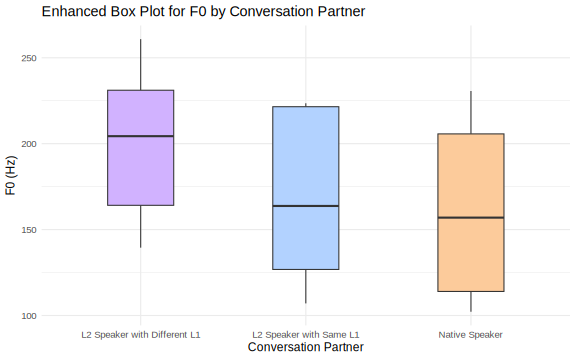
\includegraphics[keepaspectratio]{L2-clear-speech_files/figure-pdf/fig-f0-boxplot-1.pdf}}

{\noindent \emph{Note.} F0 (Hz) for each group.}

\end{figure}

\begin{figure}[!htbp]

{\caption{{F0 Range by Conversation
Partner}{\label{fig-f0range-boxplot}}}}

\pandocbounded{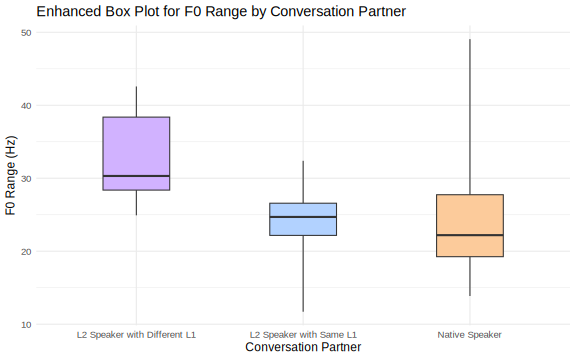
\includegraphics[keepaspectratio]{L2-clear-speech_files/figure-pdf/fig-f0range-boxplot-1.pdf}}

{\noindent \emph{Note.} F0 Range (Hz) for each group.}

\end{figure}

\begin{figure}[!htbp]

{\caption{{F0 Comparison by Gender in L2
Speakers}{\label{fig-f0-gender-difference-l2diffl1-group}}}}

\pandocbounded{\includegraphics[keepaspectratio]{L2-clear-speech_files/figure-pdf/fig-f0-gender-difference-l2diffl1-group-1.pdf}}

{\noindent \emph{Note.} F0 (Hz).}

\end{figure}

\clearpage

\section{References}\label{references}

\phantomsection\label{refs}
\begin{CSLReferences}{1}{0}
\bibitem[\citeproctext]{ref-bradlow_clear_2002}
Bradlow, A., \& Bent, T. (2002). The clear speech effect for non-native
listeners. \emph{The Journal of the Acoustical Society of America},
\emph{112}(1), 272--284. \url{https://doi.org/10.1121/1.1487837}

\bibitem[\citeproctext]{ref-calandruccio_clear-speech_2020}
Calandruccio, L., Porter, H., Leibold, L., \& Buss, E. (2020). The
clear-speech benefit for school-age children: {Speech}-in-noise and
speech-in-speech recognition. \emph{Journal of Speech, Language, and
Hearing Research}, \emph{63}(12), 4265--4276.
\url{https://doi.org/10.1044/2020_JSLHR-20-00353}

\bibitem[\citeproctext]{ref-hazan_acoustic-phonetic_2011}
Hazan, V., \& Baker, R. (2011). Acoustic-phonetic characteristics of
speech produced with communicative intent to counter adverse listening
conditions. \emph{The Journal of the Acoustical Society of America},
\emph{130}(4), 2139--2152. \url{https://doi.org/10.1121/1.3623753}

\bibitem[\citeproctext]{ref-hazan_clear_2018}
Hazan, V., Tuomainen, O., Kim, J., Davis, C., Sheffield, B., \&
Brungart, D. (2018). Clear speech adaptations in spontaneous speech
produced by young and older adults. \emph{The Journal of the Acoustical
Society of America}, \emph{144}(3), 1331--1346.
\url{https://doi.org/10.1121/1.5053218}

\bibitem[\citeproctext]{ref-jung_acoustic_2023}
Jung, Y.-J., \& Dmitrieva, O. (2023). Acoustic properties of non-native
clear speech: {Korean} speakers of {English}. \emph{Speech
Communication}, \emph{154}, 102982.
\url{https://doi.org/10.1016/j.specom.2023.102982}

\bibitem[\citeproctext]{ref-kato_perceptual_2022}
Kato, M., \& Baese-Berk, M. (2022). Perceptual consequences of native
and non-native clear speech. \emph{The Journal of the Acoustical Society
of America}, \emph{151}(2), 1246--1258.
\url{https://doi.org/10.1121/10.0009403}

\bibitem[\citeproctext]{ref-lee_maintenance_2020}
Lee, D.-Y., \& Baese-Berk, M. (2020). The maintenance of clear speech in
naturalistic conversations. \emph{The Journal of the Acoustical Society
of America}, \emph{147}(5), 3702--3711.
\url{https://doi.org/10.1121/10.0001315}

\bibitem[\citeproctext]{ref-mattys_speech_2012}
Mattys, S., Davis, M., Bradlow, A., \& Scott, S. (2012). Speech
recognition in adverse conditions: {A} review. \emph{Language and
Cognitive Processes}, \emph{27}(7-8), 953--978.
\url{https://doi.org/10.1080/01690965.2012.705006}

\bibitem[\citeproctext]{ref-picheny_speaking_1985}
Picheny, M., Durlach, N., \& Braida, L. (1985). Speaking clearly for the
hard of hearing {I}: {Intelligibility} differences between clear and
conversational speech. \emph{Journal of Speech, Language, and Hearing
Research}, \emph{28}(1), 96--103.
\url{https://doi.org/10.1044/jshr.2801.96}

\bibitem[\citeproctext]{ref-smiljanic_bidirectional_2011}
Smiljanić, R., \& Bradlow, A. (2011). Bidirectional clear speech
perception benefit for native and high-proficiency non-native talkers
and listeners: Intelligibility and accentedness. \emph{The Journal of
the Acoustical Society of America}, \emph{130}(6), 4020--4031.
\url{https://doi.org/10.1121/1.3652882}

\bibitem[\citeproctext]{ref-tuomainen_speech_2022}
Tuomainen, O., Taschenberger, L., Rosen, S., \& Hazan, V. (2022). Speech
modifications in interactive speech: Effects of age, sex and noise type.
\emph{Philosophical Transactions of the Royal Society B},
\emph{377}(1841), 20200398. \url{https://doi.org/10.1098/rstb.2020.0398}

\bibitem[\citeproctext]{ref-van_engen_wildcat_2010}
Van Engen, K., Baese-Berk, M., Baker, R., Choi, A., Kim, M., \& Bradlow,
A. (2010). The {Wildcat} {Corpus} of native-and foreign-accented
{English}: {Communicative} efficiency across conversational dyads with
varying language alignment profiles. \emph{Language and Speech},
\emph{53}(4), 510--540. \url{https://doi.org/10.1177/0023830910372495}

\end{CSLReferences}






\end{document}
